\documentclass[brazil,times]{abnt}
\usepackage[T1]{fontenc}
\usepackage[utf8]{inputenc}
\usepackage{url}
\usepackage{graphicx}
\usepackage[pdfborder={0 0 0}]{hyperref}
\usepackage{amssymb}
\usepackage{amsmath}
\usepackage[section]{placeins}
\makeatletter
\usepackage{babel}
\makeatother

\begin{document}


\autor{Pedro Paulo Vezzá Campos}

\titulo{Transcrição Automática de Música Monofônica}

\comentario{Primeiro exercício-programa apresentado para avaliação na disciplina
MAC0300, do curso de Bacharelado em Ciência da Computação, turma 45, da
Universidade de São Paulo, ministrada pelo professor Walter Figueiredo Mascarenhas.}

\instituicao{Departamento de Ciência da Computação \par Instituto de Matemática
e Estatística \par Universidade de São Paulo}

\local{São Paulo - SP, Brasil}

\data{\today}

\capa

\folhaderosto

\tableofcontents

\chapter{Introdução\label{cap:introducao}}
	Neste primeiro exercício-programa de MAC0300 - Métodos Numéricos da Álgebra Linear foi pedido que implementássemos um programa que fosse capaz de realizar a transcrição automática de músicas simples, ou seja, transformar um arquivo WAV contendo sons monofônicos em um arquivo MIDI equivalente. Neste relatório serão apresentados: Uma explicação da modelagem de sons utilizando Séries de Fourier, explicações sobre a Transformada de Fourier e suas duas principais implementações (DFT e FFT), uma análise dos resultados obtidos com o programa em termos das Transformadas utilizadas e do tempo de execução, por fim, será feita apresentada uma conclusão sobre o EP.

% Explique sucintamente a modelagem de um som usando Série de Fourier;
\chapter{Modelagem de som usando Séries de Fourier}
	Para modelar uma onda sonora matematicamente, primeiramente precisamos definir o que vem a ser o som. Segundo \cite{ufpe:computacao-musical}, o som é uma "forma de energia mecânica que se propaga causando compressão e rarefação das moléculas de um meio elástico e inercial (Sólido, líquido ou gasoso)". Por ser uma onda mecânica, possui características comuns a tais ondas, tais como: amplitude, freqüência, comprimento, velocidade, fase, potência, etc. Isso nos permite deduzir uma forma de estudar o som utilizando o arcabouço vindo do campo da Ondulatória.
	
	Uma onda sonora simples pode, então, ser descrita como uma senoide da forma $x(t) = A \operatorname{sen} (ft + \theta)$ onde $A$ é a amplitude, $f$ é a freqüência e $\theta$ é a fase inicial.

	Jean Baptiste Fourier (1768 - 1830) percebeu que toda onda periódica pode ser expressa como uma soma infinita de ondas senoidais de amplitudes variadas. Ainda, as frequências de tais senoides devem ser múltiplas inteiras de alguma frequência fundamental. A esta soma infinita dá-se o nome de Série de Fourier. \cite{burk2005music} Mais formalmente, segundo \cite{wiki:serie-fourier} tomemos $f(x)$ periódica, ou seja:


	$$f(t + 2L) = f(t), \quad c \le t \le c + 2L$$

	Então:

	$$f(t) = a_k + a_0\operatorname{sen}(f_0t + \theta 0) +... + a_n\operatorname{sen} (f_nt + \theta n)$$


	Para a representação de funções não-periódicas, lançamos mão da Transformada de Fourier, que estudará o sinal no seu espectro de frequências. Tal assunto será discutido em seguida.

\chapter{Transformada de Fourier}
	A Transformada de Fourier (TF) é uma operação matemática responsável por expressar uma função de domínio o tempo (No SI, segundos) como uma função de domínio na frequência (No SI, hertz). Sua função é decompor um sinal em suas componentes elementares, seno e cosseno. \cite{ufcg:transformada-fourier} No estudo de sons, a TF de uma nota musical é uma representação matemática das amplitudes e fases nas notas individuais que a compõem. Cada valor retornado pela transformada é usualmente expresso como um número complexo (Conhecido como amplitude complexa) que pode ser interpretado como duas componentes, a magnitude e a fase de uma dada frequência.


	\section{Transformada Contínua de Fourier}
		A Transformada de Fourier $\hat{f}$ de uma função integrável $f: R \rightarrow C$ é definida como \cite{wiki:fourier-transform}:

		$$\hat{f}(\xi) = \int_{-\infty}^{\infty} f(x)\ e^{- 2\pi i x \xi}\,dx \text{, para todo número real } \xi.$$

		Se a variável independente $x$ representa uma unidade de tempo, a variável da transformada $\xi$ representa uma unidade de frequência. 
		
		Esta forma de cálculo da TF é inviável computacionalmente por depender de uma integração imprópria de uma função contínua, o que necessitaria de cálculos infinitesimais para formar o resultado exato. Porém, através da amostragem de um sinal contínuo podemos aplicar a Transformada Discreta de Fourier.

	\section{Transformada Discreta de Fourier}
		Caso a função a ser transformada seja discreta e de duração finita (Ou periódica) é possível deduzir uma versão discreta da Transformada de Fourier (DFT):

		$$X_k = \sum_{n=0}^{N-1} x_n \cdot e^{-i 2 \pi \frac{k}{N} n}.$$

		Agora, a entrada da transformada é uma sequência finita de números reais ou complexos, isso a torna ideal para o processamento de informação armazenada em computadores. Em particular, a DFT é largamente empregada em processamento de sinais e outros campos relacionados para analisar frequências contidas em um sinal amostrado, resolver equações diferenciais parciais ou realizar multiplicações de inteiros grandes. O cálculo da DFT pode ser feito de diversas formas, que diferem na complexidade da operação ($O(n^2)$) ou ($O(n \log{n})$) e na precisão dos resultados gerados. Tais detalhes serão explicados posteriormente.



% Descreva vantagens e desvantagens entre os métodos Multiplicação pela Matriz de Fourier e FFT.
\chapter{Métodos para implementar a Transformada de Fourier}
	Nesta seção apresentaremos dois métodos de calcular a DFT, utilizando uma matriz DFT e através da Transformada Rápida de Fourier (FFT). Posteriormente faremos uma comparação de ambos os métodos.
	
	\section{Matriz DFT}
		Esta é a maneira de implementar "ingenuamente" a DFT. Ela é realizada através do produto

		$$T = \mathbf{F}x \text{, onde $T$ é a transformada do sinal $x$ de dimensão $N$ e $\mathbf{F}$ é matriz:}$$

		$$
		\mathbf{F} =
		\begin{bmatrix}
			\omega_N^{0 \cdot 0}     & \omega_N^{0 \cdot 1}     & \ldots & \omega_N^{0 \cdot (N-1)}     \\
			\omega_N^{1 \cdot 0}     & \omega_N^{1 \cdot 1}     & \ldots & \omega_N^{1 \cdot (N-1)}     \\
			\vdots                   & \vdots                   & \ddots & \vdots                       \\
			\omega_N^{(N-1) \cdot 0} & \omega_N^{(N-1) \cdot 1} & \ldots & \omega_N^{(N-1) \cdot (N-1)} \\
		\end{bmatrix}
		$$

		$$\omega_N = e^{-2 \pi i/N}\,$$


		Como estamos realizando um produto-matriz vetor, no qual a dimensão de $x$ é $N$, a complexidade do produto é dado por $O(N^2)$

	\section{Transformada Rápida de Fourier}
		Através de uma estratégia de divisão-e-conquista é possível atingir o mesmo resultado obtido pela matriz DFT com uma complexidade dos cálculos menor, de $O(N^2)$ para $O(N\log{N})$. O método mais utilizado para o cálculo da FFT é o Algoritmo de Cooley-Tuckey. Ele divide o cálculo da transformada recursivamente de um sinal discreto de tamanho $N = N_1 N_2$ nas parcelas $N_1$ e $N_2$.
		
		Tal método foi popularizado por um artigo de J. W. Cooley e J. W. Tukey em 1965, porém tal método já era conhecido por Gauss em 1805. O interesse pelo método foi num momento de popularização dos computadores para cálculos científicos e militares, o que permitiu gerar resultados mais rapidamente que previamente. A versão mais famosa do algoritmo, que divide o cálculo em duas partes iguais (E portanto exigindo que o sinal tenha dimensão uma potência de 2) vista em \cite{wiki:cooley-tukey}.


	\section{Comparação entre a Matriz DFT e a FFT}
		A diferença mais impactante entre os dois métodos já foi comentada: Enquanto o método de multiplicação pela Matriz DFT consome tempo $O(N^2)$, uma FFT necessita de tempo $O(N\log{N})$ para o mesmo cálculo. Isso é extremamente importante pois usualmente sinais possuem quantidades da ordem de dezenas ou centenas de milhares de amostras, o que faz com que o tempo necessário entre um e outro método varie possivelmente em algumas ordens de grandeza, como será visto mais à diante na seção de resultados experimentais do EP.
	
		Porém, o método de multiplicação tem como vantagem o fato de aceitar sinais com qualquer quantidade de amostras, diferentemente de algoritmos famosos de FFT como o Cooley-Tuckey comentado anteriormente. Este, na sua versão mais famosa, exige que o sinal possua uma quantidade de amostras potência de 2 para funcionar corretamente. A consequência disso é que o método da multiplicação pode ser mais preciso nos resultados que uma FFT, conforme detalha \cite{voltech:dft-vs-fft}.
		
		O efeito em que os dados de amplitude e fase aparecem na frequência errada após o cálculo da FFT é conhecido como ``spectral leakage''. Há soluções para este problema como por exemplo o uso de ``janelas'' no sinal a ser amostrado. Um outro detalhe que influi na escolha do algoritmo é o conhecimento prévio do sinal a ser quantizado. Caso saiba-se quantas harmônicas há em um sinal podemos excluir do cálculo da Matriz DFT a quantização de frequências desnecessárias. Isso traz um grande ganho de velocidade ao método da Matriz DFT, permitindo unir o melhor dos dois mundos: Precisão e velocidade nos cálculos da transformada.
	

% Explique como a Transformada de Fourier fornece informações para a transcrição musical feita em seu programa;
\chapter{Transformada de Fourier na transcrição musical}
	O som pode ser interpretado, como foi visto anteriormente, como um sinal contínuo composto por uma ou mais senoides de diferentes frequências e amplitudes. Sendo assim, é passível de ser mapeado em seu respectivo espectro de frequências através da Transformada de Fourier. No caso do EP, foi requisitado que convertessemos arquivos .wav (Ou seja, som amostrado 44100 vezes por segundo) contendo notas musicais e possivelmente hamônicos e/ou ruídos. A tarefa era detectar a(s) frequência(s) fundamental(is) do intervalo e gravar tal(is) frequência(s) como evento(s) MIDI.

	Para resolver este problema a Transformada de Fourier foi fundamental pois com o espectro do sinal sonoro é relativamente simples descobrirmos qual é a frequência fundamental. Como pedido no enunciado, foram empregadas as duas estratégias de DFT descritas neste relatório, o método de multiplicação por Matriz DFT e FFT. O algoritmo descrito em alto nível do EP ficou assim:
	
	{\scriptsize
    \begin{verbatim}
        y <- le_wav(arquivo) /* Extraímos o sinal amostrado do arquivo .wav */
        tempos <- determina_tempos(y) /* Vetor que indica na posição i quantas notas já tocaram */
        midi <- criar_midi()
        para cada nova nota 'n' tocada, faça:
            inicio <- inicio_nota(n, tempos) /* Instante de início da nota (em segundos) */
            fim <- fim_nota(n, tempos);/* Instante de término da nota (em segundos) */
            x <- transformada(y(n, n + 1)) /* Matriz DFT ou FFT. Analisamos apenas 1 segundo, 
                                            o que é suficiente pelas restrições do EP.*/
            amp <- amplitudes(x) /* Transforma o vetor x de números complexos em reais */
            mediana <- mediana(amp)
            desvio <- desvio_padrao(amp)
            eventos = {}
            para cada i em [1 .. |amp|] faça
                a <- amp(i)
                f <- i *  44100 / |amp|
                se a > mediana + 3 * desvio então
                    evento <- freq_para_midi(f)
                    evento = eventos U {evento}
                fim se
            fim para
            
            /* Vamos filtrar eventos encontrados em busca da nota com mais harmônicas
            Pela tabela de eventos MIDI percebe-se que as harmônicas de um evento e
            são iguais a: e + n * 12, com n inteiro. Para isso vamos colocar cada evento
            em na sua classe de congruência mod 12 e acumular as amplitudes de cada evento
            no sinal amostrado. Aquela classe que tiver mais harmônicas (Ou maior amplitude
            no caso de empate) tem grandes chances de conter a frequência fundamental */
            
            cont_harmonicas <- zeros(1, 12)
            acc_amplitudes <- zeros(1, 12)
            para cada evento em eventos
                cont_harmonicas((evento mod 12) + 1) += 1
                acc_amplitudes((evento mod 12) + 1) += amplitudes(floor(
                    midi_para_freq(evento) * |amp| / 44100))
            endfor
            
            classe_fundamental <- mais_harmonicas_maior_amp(cont_harmonicas, acc_amplitudes, eventos)
                /* Retorna os eventos correspondentes à classe da fundamental segundo
                    o critério acima */
            fundamental <- min(ordene(classe_fundamental))
            escreva_evento(midi, fundamental, inicio, fim)
        fim para
    \end{verbatim}}


% Mostre os gráficos das ondas de áudio no domínio do tempo e no domínio da frequência (frequência no eixo das abscissas e amplitude em decibéis no eixo das ordenadas). Mostre os espectros obtidos para ambos os métodos.
\chapter{Gráficos dos resultados obtidos}
	Nesta seção serão apresentados alguns gráficos no domínio do tempo e da frequência extraídos da execução do programa. Foram produzidos gráficos para todos os arquivos .wav fornecidos com o enunciado. Eles estão no diretório graficos do pacote contendo o código fonte e relatório.

	\section{Domínio do tempo}
		No eixo das abcissas está o tempo em segundos e no eixo das ordenadas estão as amostras em codificação linear (Valores entre -1 e 1).
			%\usepackage{graphics} is needed for \includegraphics
			\begin{figure}[h!]
			\begin{center}
			  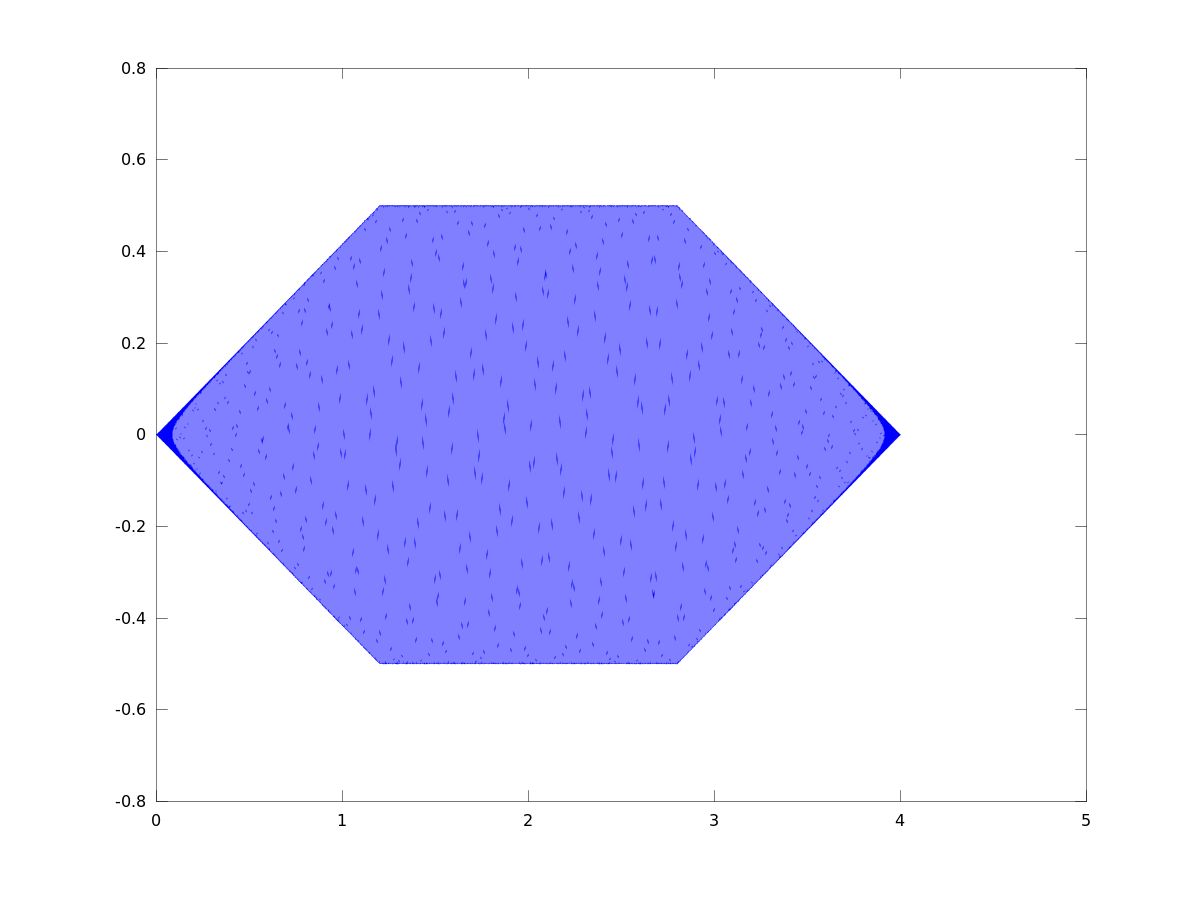
\includegraphics[width=150mm]{imagens/1notaA4_tempo.png}
			  \caption[1notaA4.wav]{1notaA4.wav}
			\end{center}
			\end{figure}

			%\usepackage{graphics} is needed for \includegraphics
			\begin{figure}[h!]
			\begin{center}
			  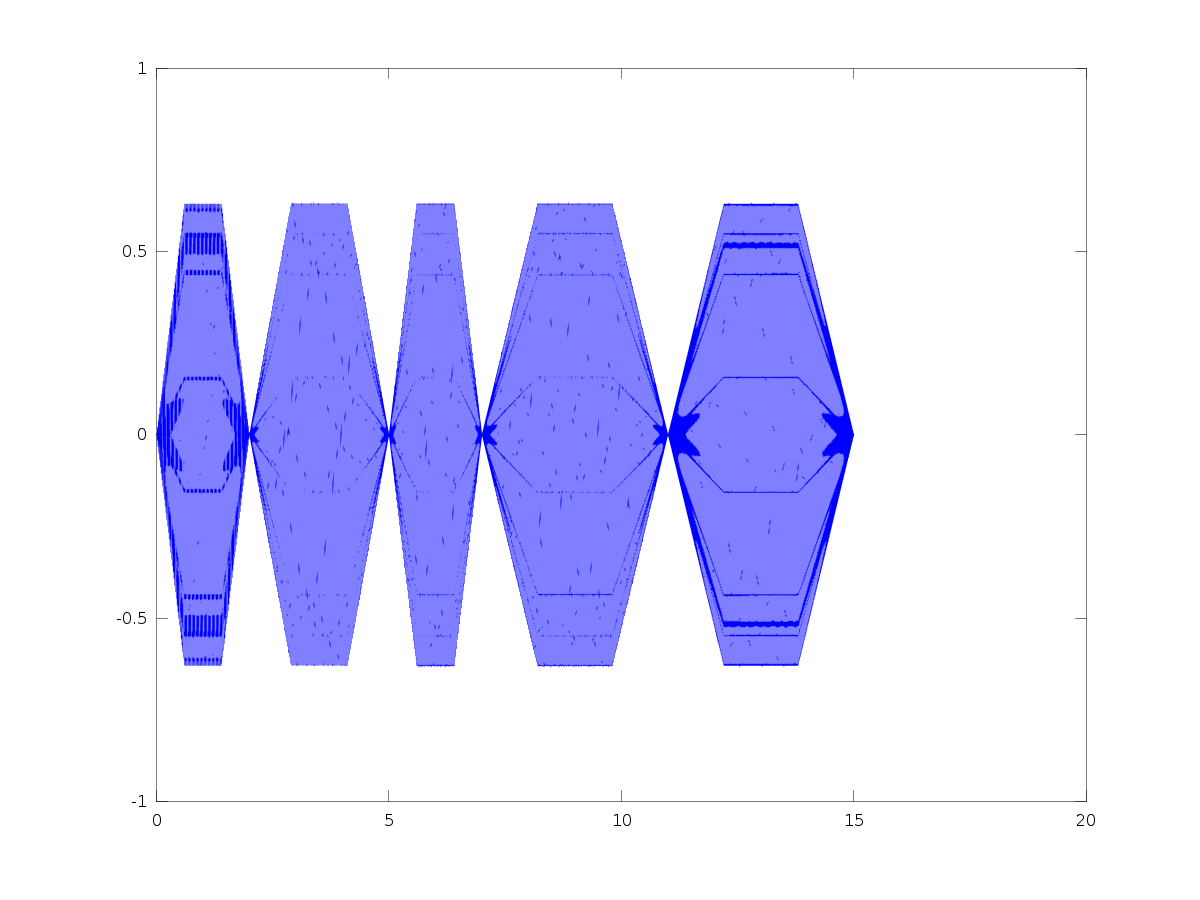
\includegraphics[width=150mm]{imagens/34_60_57_56_43_4harmonicos_tempo.png}
			  \caption[34\_60\_57\_56\_43\_4harmonicos.wav]{34\_60\_57\_56\_43\_4harmonicos.wav}
			\end{center}
			\end{figure}

			%\usepackage{graphics} is needed for \includegraphics
			\begin{figure}[h!]
			\begin{center}
			  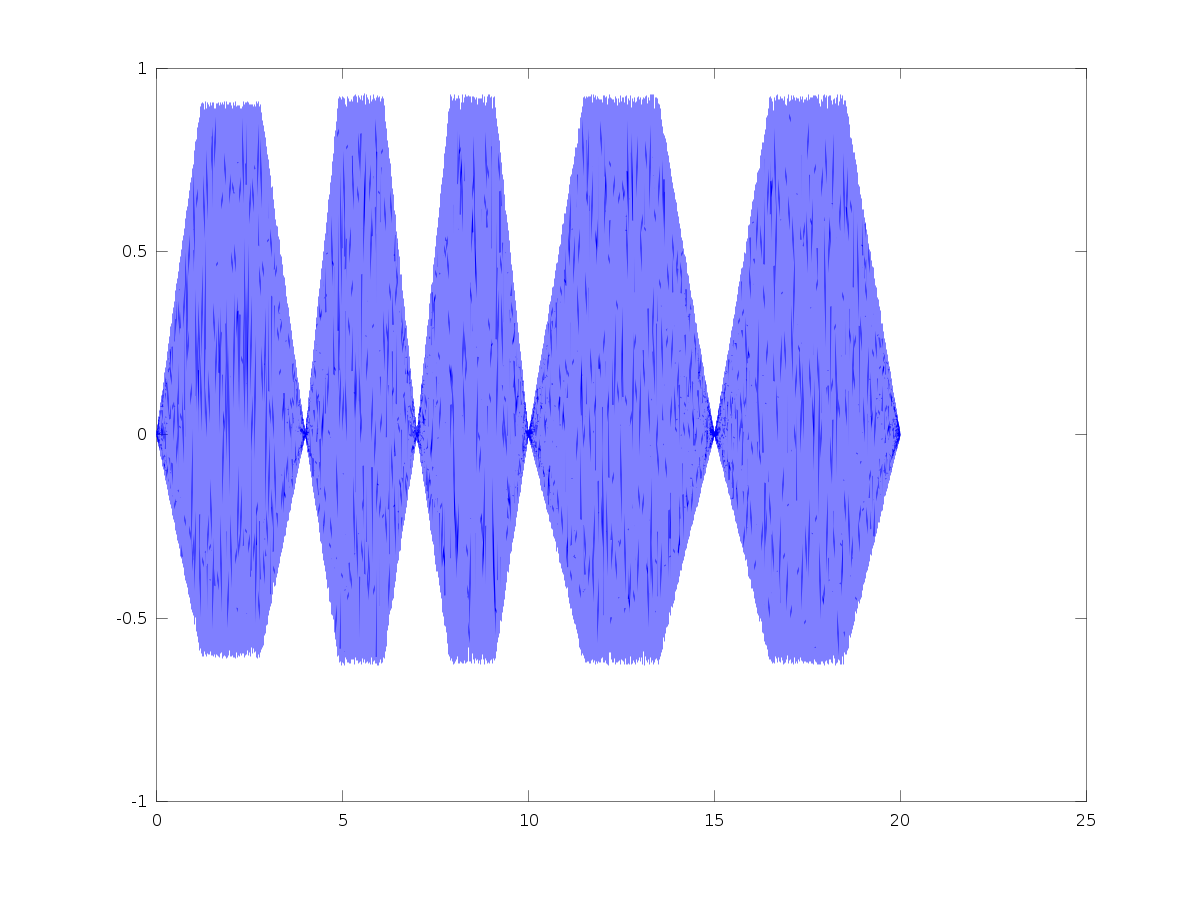
\includegraphics[width=150mm]{imagens/95_81_79_77_76_4harms_com_ruido_tempo.png}
			  \caption[95\_81\_79\_77\_76\_4harms\_com\_ruido.wav]{95\_81\_79\_77\_76\_4harms\_com\_ruido.wav}
			\end{center}
			\end{figure}

	\section{Domínio da frequência}
		No eixo das abcissas está a frequência em hertz e no eixo das ordenadas está a amplitude em decibéis.

			%\usepackage{graphics} is needed for \includegraphics
			\begin{figure}[h!]
			\begin{center}
			  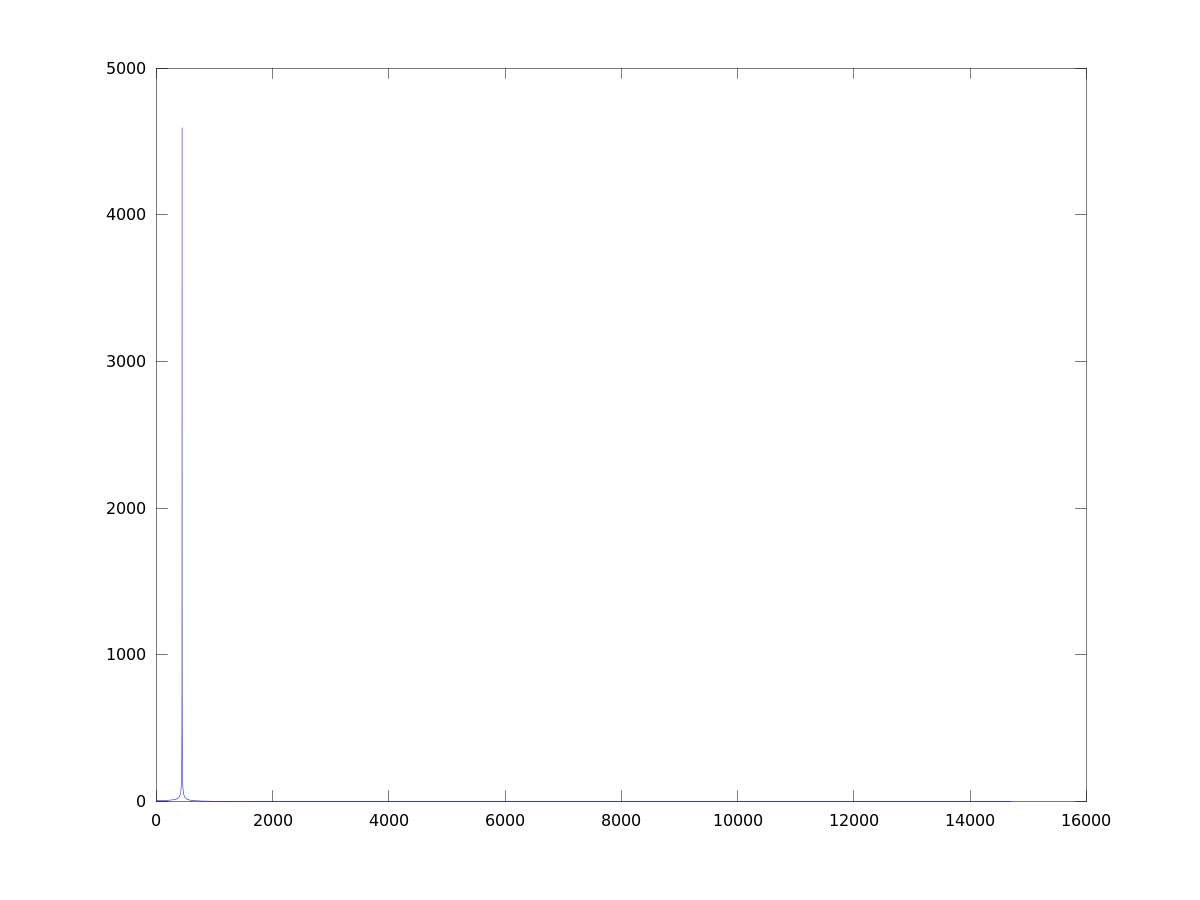
\includegraphics[width=150mm]{imagens/1notaA4_freq_seg_1.png}
			  \caption[1notaA4.wav - Primeiro segundo]{1notaA4.wav - Primeiro segundo}
			\end{center}
			\end{figure}

			%\usepackage{graphics} is needed for \includegraphics
			\begin{figure}[h!]
			\begin{center}
			  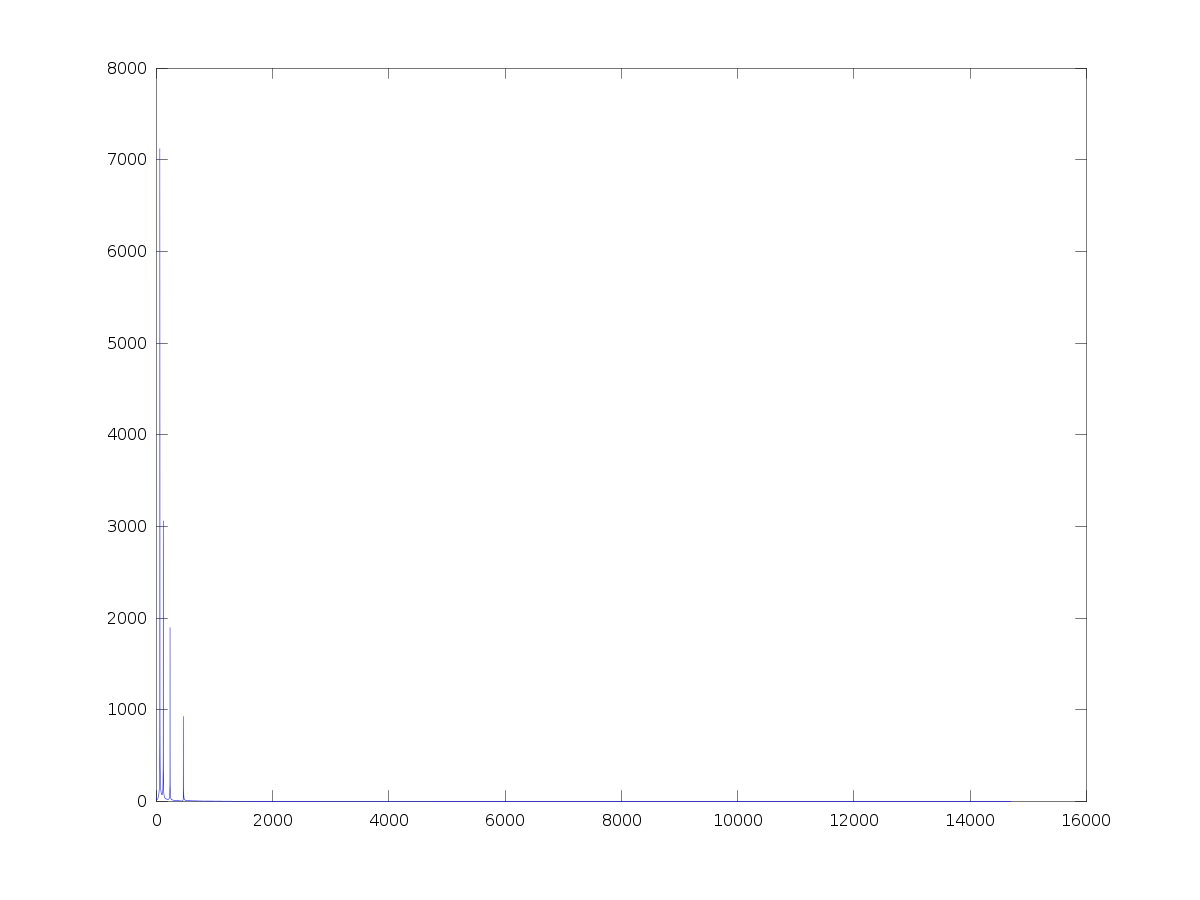
\includegraphics[width=150mm]{imagens/34_60_57_56_43_4harmonicos_freq_seg_1.png}
			  \caption[34\_60\_57\_56\_43\_4harmonicos.wav - Primeiro segundo]{34\_60\_57\_56\_43\_4harmonicos.wav - Primeiro segundo}
			\end{center}
			\end{figure}
			
			%\usepackage{graphics} is needed for \includegraphics
			\begin{figure}[h!]
			\begin{center}
			  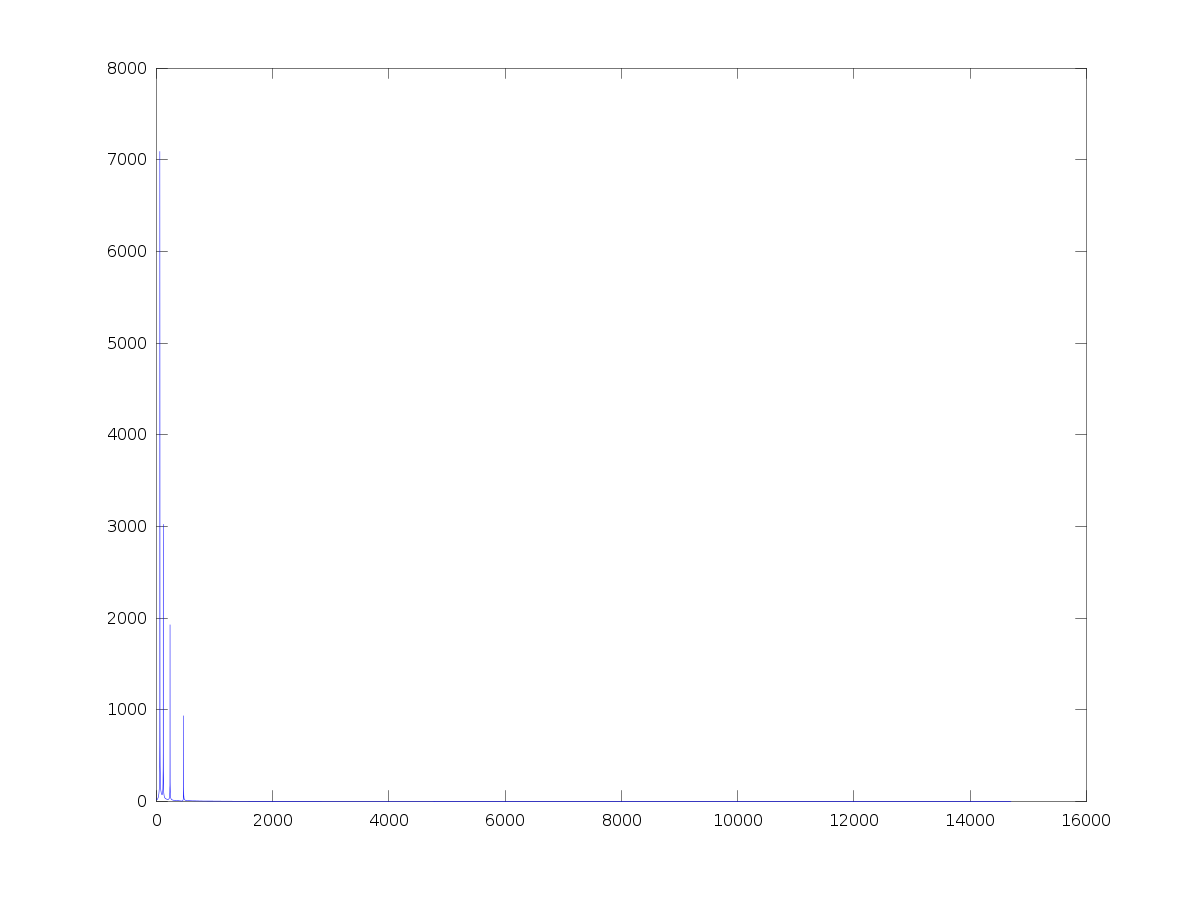
\includegraphics[width=150mm]{imagens/34_60_57_56_43_4harmonicos_freq_seg_2.png}
			  \caption[34\_60\_57\_56\_43\_4harmonicos.wav - Segundo segundo]{34\_60\_57\_56\_43\_4harmonicos.wav - Segundo segundo}
			\end{center}
			\end{figure}

			%\usepackage{graphics} is needed for \includegraphics
			\begin{figure}[h!]
			\begin{center}
			  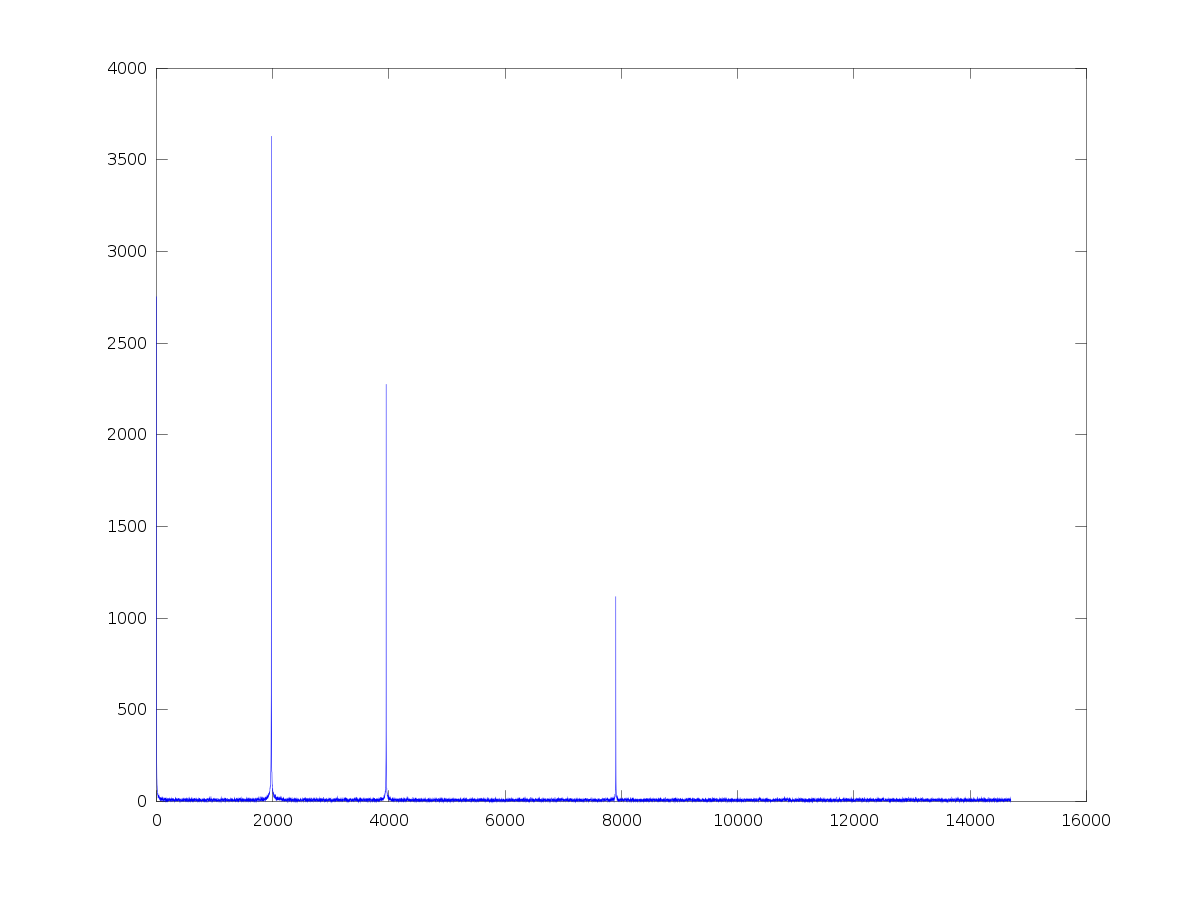
\includegraphics[width=150mm]{imagens/95_81_79_77_76_4harms_com_ruido_freq_seg_1.png}
			  \caption[95\_81\_79\_77\_76\_4harms\_com\_ruido.wav - Primeiro segundo]{95\_81\_79\_77\_76\_4harms\_com\_ruido.wav - Primeiro segundo}
			\end{center}
			\end{figure}

			%\usepackage{graphics} is needed for \includegraphics
			\begin{figure}[h!]
			\begin{center}
			  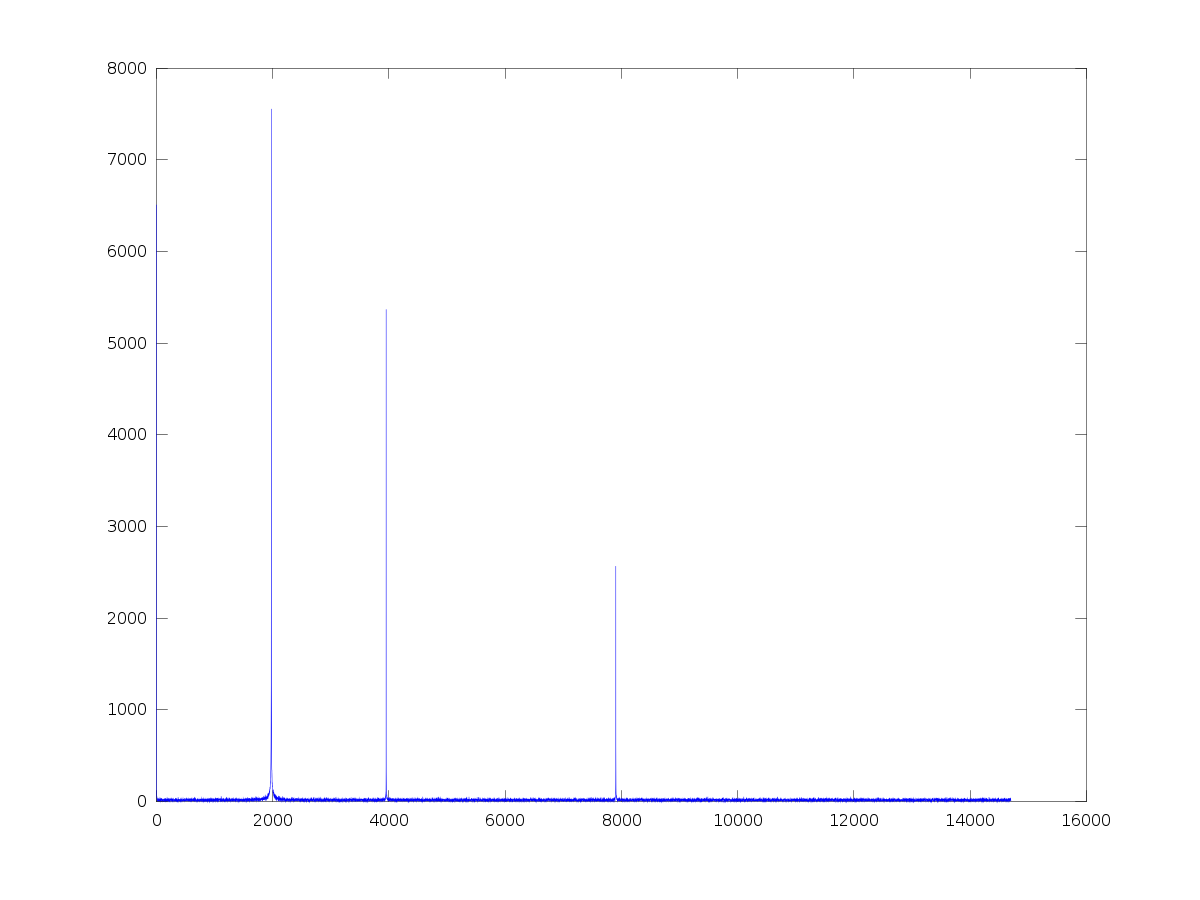
\includegraphics[width=150mm]{imagens/95_81_79_77_76_4harms_com_ruido_freq_seg_2.png}
			  \caption[95\_81\_79\_77\_76\_4harms\_com\_ruido.wav - Segundo segundo]{95\_81\_79\_77\_76\_4harms\_com\_ruido.wav - Segundo segundo}
			\end{center}
			\end{figure}

% Faça a comparação do tempo de execução dos dois métodos de cálculo da Transformada Discreta de Fourier: Multiplicação pela Matriz de Fourier e FFT. Mostre dois gráficos comparativos com os tempos médios dos métodos para o mesmo número de execuções. Tome o cuidado de não incluir o tempo de criação da matriz DFT no método da multiplicação.
\chapter{Análise dos tempos de execução do programa}
Nesta seção vamos comparar os tempos de execução do programa utilizando o método da multiplicação por Matriz DFT e FFT. A expectativa é evidenciar a diferença na complexidade computacional dos dois métodos. A medição do tempo não inclui a geração da matriz DFT, apenas o produto descrito anteriormente. 

Os testes foram realizados em um PC utilizando um processador Core i5 rodando Debian GNU/Linux. Os resultados condizem com a expectativa, a FFT é ordens de grandeza mais rápida que a matriz DFT, levando sempre menos que 1 segundo para realizar todos os cálculos necessários. Pela curva desenhada no gráfico da DFT vemos que realmente há um aumento substancial no tempo de execução do programa à medida que aumenta-se o tamanho do arquivo a ser processado, porém menor que um aumento quadrático. Enquanto um arquivo de 1 segundo de áudio demora aproximadamente 400 segundos para executar via matriz outro de 5 segundos de áudio leva 1400 segundos, aumento de 3,5 vezes. A diferença entre o aumento experado e real pode ser explicado por otimizações que o octave e o microcódigo do processador realizam internamente para explorar ao máximo o paralelismo disponível na máquina.

\begin{table}	
    \begin{tabular}{|l|l|l|l|}
        \hline
		Arquivo & Música (s) & DFT (s) & FFT (s) \\ \hline
		1notaA4\_1seg\_4harmonicos2 & 1 & 389.13 & 0.092826 \\
		1notaA4\_1seg\_4harmonicos3 & 1 & 429.11 & 0.1083 \\
		1notaA4\_1seg\_4harmonicos & 1 & 388.31 & 0.10788 \\
		1notaA4\_1seg & 1 & 394.09 & 0.10506 \\
		1notaA4 & 4 & 1166.1 & 0.10961 \\
		41\_97\_23\_73\_56\_1seg\_4harmonicos & 5 & 1396.4 & 0.084259 \\
		53\_35\_94\_35\_107\_1seg & 5 & 1458.5 & 0.12121 \\
		5notas1segA4 & 5 & 1408.5 & 0.12008 \\
		5notas1segC4 & 5 & 1474.1 & 0.10318 \\
		5notas1segE4 & 5 & 1420.6 & 0.10345 \\
		95\_85\_62\_102\_52\_1seg & 5 & 1387.4 & 0.092917 \\
		75\_77\_100\_84\_73\_1seg & 5 & 1379.2 & 0.088239 \\
		57\_91\_98\_84\_26\_4harmonicos & 9 & 1893.2 & 0.10231 \\
		64\_75\_27\_29\_84\_4harmonicos & 14 & 2525.1 & 0.1001 \\
		34\_60\_57\_56\_43\_4harmonicos & 15 & 2859.8 & 0.12572 \\
		5notasC4 & 16 & 2868 & 0.12522 \\
		5notasE4 & 17 & 2915.2 & 0.1117 \\
		50\_85\_63\_96\_100 & 18 & 2986 & 0.1344 \\
		82\_93\_107\_61\_81 & 18 & 2812.9 & 0.1187 \\
		39\_39\_97\_77\_41\_3harmonicos & 19 & 2996.2 & 0.12426 \\
		5notasA4 & 20 & 3076.3 & 0.12708 \\
		95\_81\_79\_77\_76\_4harms\_com\_ruido & 20 & 2772 & 0.11912 \\
        \hline
    \end{tabular}
\end{table}


	%\usepackage{graphics} is needed for \includegraphics
	\begin{figure}[h!]
	\begin{center}
	  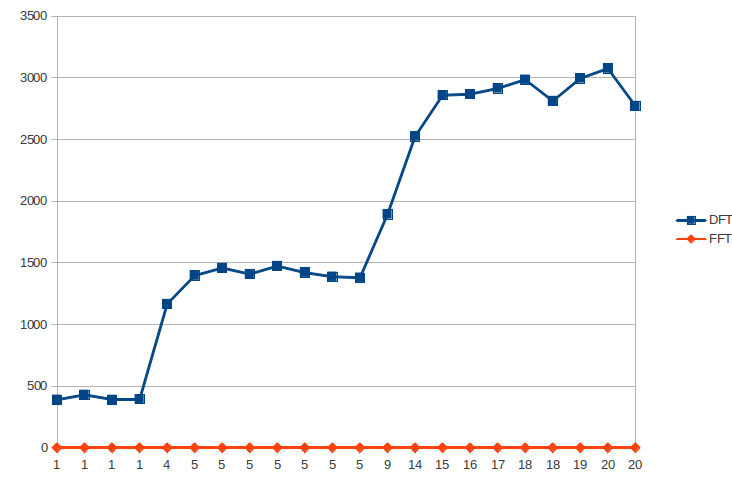
\includegraphics[width=150mm]{imagens/tempos.png}
	  \caption[Grático dos tempos de execução com matriz DFT e FFT]{Grático dos tempos de execução com matriz DFT e FFT}
	\end{center}
	\end{figure}


\chapter{Conclusão}
	O trabalho ajudou a fixar os conceitos vistos em aula, além de nos fazer entrar em contato com uma área não habitualmente abordada na graduação, Processamento de Sinais. Os alunos tiveram um contato prático com os conceitos, com a teoria relacionada sendo estudada à medida que havia necessidade de interpretar os resultados obtidos. Isso permitiu acumular diversos conhecimentos úteis enquanto resolve-se um problema real na área de Computação Musical. Ainda, a possibilidade de utilizar uma linguagem voltada pra processamentos matemáticos, tal como Octave, a escolhida para este trabalho, simplificou problemas de implementação, permitindo aos alunos focarem nos algoritmos propriamente ditos. Vencida a dificuldade com o entendimento do problema a ser resolvido e questões de representação de números de ponto flutuante e complexos o EP foi bastante interessante de ser implementado.
	
\nocite{*}
\bibliographystyle{abnt-num}
\bibliography{bibliografia}
\end{document}

\end{document}
